\chapter{Setup}
All experiments are done within the Cooja simulator. The environment we simulated is as described in \Cref{fig: Setup}.

\begin{figure}
\centering
{
	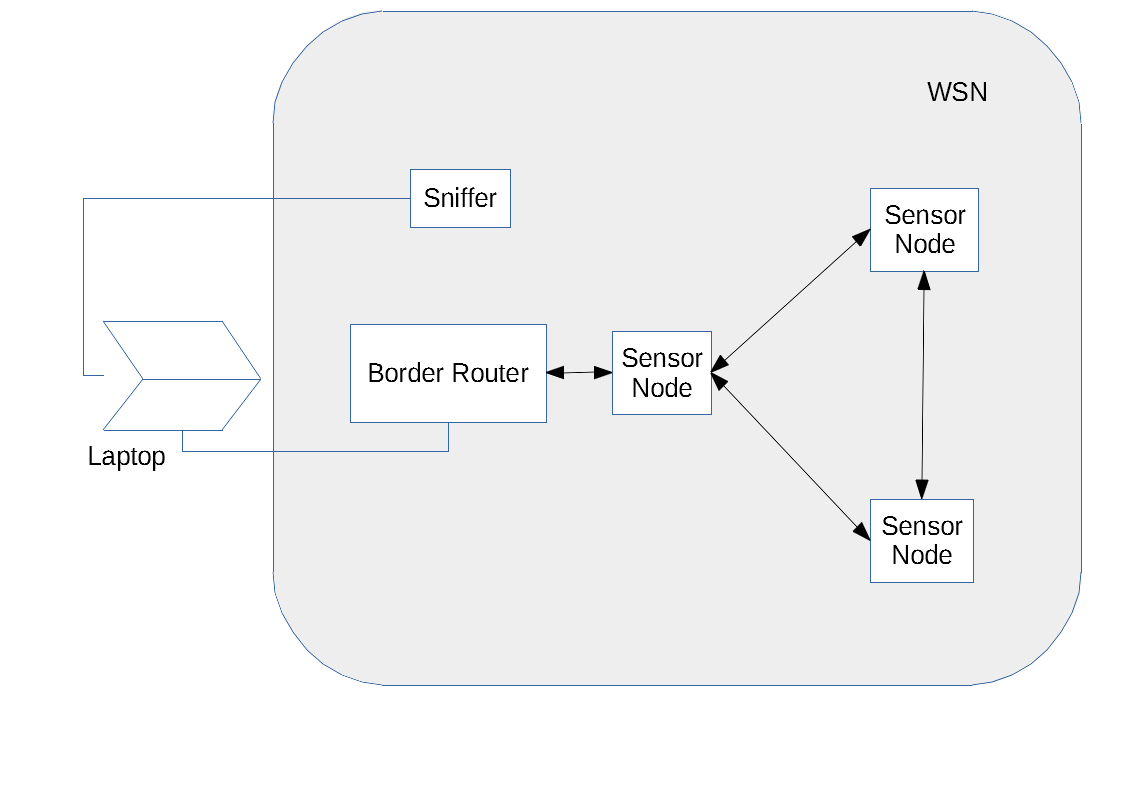
\includegraphics[width=0.7\textwidth,]{fig/setup.png}
}
\caption{Experiment setup} \label{fig: Setup}
\end{figure}

\begin{itemize}
\item{\bf Adversary} is a malicious party that tries to illegally reveal information from the encrypted traffic.
\item{\bf Border Router}, or BR, is a device that connects adversary to the sensor network. \textbf{BR is not allowed when LLSEC is enabled} as the adversary does not have the key and hence cannot connect into the network. We will discuss more about LLSEC in \Cref{Chp: LLSEC}.
\item{\bf Sniffer} passively captures all traffic in the network. 
\item{\bf Target} and {\bf Nodes} are sensors deployed in the sensor network. They communicates to each other through encrypted channels.
\item{\bf Sensor Network} discussed in this paper is a 6LowPAN network based on Contiki OS.
\end{itemize}

Realistically speaking, this scenario could happen say an adversary sitting near a smart house with a laptop attached to a SoC\footnote{System on Chip} device, or your malicious neighbour walks into your smart house with her smart phone.

\section{Adversary Power}
The powers assumed in the experiments are considered to be practical in real life.

When LLSEC is enabled, all traffic, including RPL\footnote{Routing Procol for Low-power and Lossy Networks} messages, are encrypted; therefore no external nodes can connect to the network as an external node cannot send any valid RPL messages to join the network. The adversary only passively sniffs all traffic.

With LLSEC disabled, the adversary can therefore join the sensor network through a BR and hence is also capable to send messages to the target(s). However, she will not be able to inject any message into an encrypted channel such as a DTLS channel.

\section{Types of Packets}
We simply categorise the packets into two types:
\begin{itemize}
\item {\bf Network Management Packets}: These are the packets generated by the protocols to  maintain the functionality of network, such as MAC ACKs, RPL messages or ICMP messages.
\item {\bf Data Packets}: These are those packets generated by applications running on sensor nodes., such as a CoAP packet.
\end{itemize}

This is only a subjective rough categorisation and may not be precise. For example an TCP data packet may set its ACK flag, or DTLS handshake packets could ambiguously fall into both categories. However, we ignore this ambiguity as it is not our focus.